% ============================================================
%  REPORTE TÉCNICO: Clasificación de Texto con Redes Neuronales
%  Dataset: 20 Newsgroups (Dataset 3) | Framework: Keras / TensorFlow
%  Curso: Redes Neuronales - Universidad del Valle (2026-2)
%  Entrega 1: Perceptrón Multicapa (MLP)
% ============================================================
\documentclass[12pt, a4paper]{article}

% ── Paquetes ────────────────────────────────────────────────
\usepackage[utf8]{inputenc}
\usepackage[T1]{fontenc}
% es-nodecimaldot: punto decimal en todo el documento (antes el texto en modo matemático usaba coma y las tablas punto)
\usepackage[spanish, es-tabla, es-nodecimaldot]{babel}
\usepackage[margin=2.5cm]{geometry}
\usepackage{lmodern}
\usepackage{microtype}

% Matemáticas
\usepackage{amsmath, amssymb}

% Gráficos y figuras
\usepackage{graphicx}
% Figuras generadas por el código del repositorio
\graphicspath{{figuras/}}
% Tablas que se reducen solo si son más anchas que la página
\usepackage{adjustbox}
\usepackage{float}
\usepackage{subcaption}

% Tablas
\usepackage{booktabs}
\usepackage{array}
\usepackage{multirow}

% Código fuente
\usepackage{listings}
\usepackage{xcolor}

% Hipervínculos
\usepackage[colorlinks=true, linkcolor=blue, citecolor=blue, urlcolor=blue]{hyperref}

% Encabezados y pies de página
\usepackage{fancyhdr}
\pagestyle{fancy}
\fancyhf{}
\rhead{\small Clasificación de Texto con MLP (Keras)}
\lhead{\small Reporte Técnico --- Entrega 1}
\cfoot{\thepage}

% Espaciado entre párrafos
\setlength{\parskip}{6pt}
\setlength{\parindent}{0pt}

% ── Estilo para código Python ────────────────────────────────
\definecolor{codegray}{rgb}{0.95,0.95,0.95}
\definecolor{codegreen}{rgb}{0.1,0.5,0.1}
\definecolor{codepurple}{rgb}{0.4,0.0,0.6}
\definecolor{codeblue}{rgb}{0.0,0.2,0.6}

\lstdefinestyle{pythonstyle}{
    backgroundcolor=\color{codegray},
    commentstyle=\color{codegreen}\itshape,
    keywordstyle=\color{codeblue}\bfseries,
    stringstyle=\color{codepurple},
    basicstyle=\ttfamily\footnotesize,
    breakatwhitespace=false,
    breaklines=true,
    captionpos=b,
    keepspaces=true,
    numbers=left,
    numberstyle=\tiny\color{gray},
    numbersep=8pt,
    showspaces=false,
    showstringspaces=false,
    showtabs=false,
    tabsize=4,
    frame=single,
    rulecolor=\color{gray!40},
    language=Python
}
\lstset{style=pythonstyle}

% ── Datos del documento ──────────────────────────────────────
\title{
    \textbf{Clasificación Multiclase de Texto en 20 Newsgroups:} \\
    \large Diseño, Regularización y Evaluación de un Perceptrón Multicapa (MLP) \\
    mediante Representaciones TF-IDF en Keras \\[1em]
 
}
\author{
    John Ramos - 2370742\\
    Kevin Ramirez - 2324793 \\
    Dylan Morales - 2328330 \\\\
    \small Escuela de Ingeniería de Sistemas y Computación \\ Universidad del Valle\\
    \small \texttt{ramos.john@correounivalle.edu.co} \\
    \small \texttt{kevin.amaya@correounivalle.edu.co} \\
    \small \texttt{dylan.morales@correounivalle.edu.co}
}
\date{\today}

% ============================================================
\begin{document}

\maketitle
\thispagestyle{fancy}

% ── RESUMEN ─────────────────────────────────────────────────
\begin{abstract}
Este reporte documenta el diseño, implementación y evaluación experimental de un Perceptrón Multicapa (MLP) desarrollado con el framework \textbf{Keras/TensorFlow} para la clasificación multiclase de documentos de texto correspondientes al conjunto de datos \textbf{20 Newsgroups} (Dataset~3). Dada la naturaleza no estructurada y dispersa del lenguaje natural, se implementó un pipeline de procesamiento lingüístico basado en vectorización \textbf{TF-IDF} con escalamiento sublineal y filtrado riguroso de metadatos (\textit{headers}, \textit{footers} y \textit{quotes}) para prevenir el fenómeno de fuga de información (\textit{data leakage}). Se diseñó y entrenó una arquitectura densa con activaciones no lineales \textbf{ReLU}, regularización mediante \textbf{Dropout}, penalización de pesos $L_2$ y una capa de salida \textbf{Softmax} de $20$ unidades. Se condujo un estudio comparativo entre dos configuraciones de red (\textbf{MLP Baseline} y \textbf{MLP Tuned}), analizando cuantitativamente la evolución de las curvas de pérdida y exactitud a lo largo de las épocas, así como métricas de desempeño globales ($F_1$-score macro, precisión y exhaustividad). Los resultados muestran que ampliar el vocabulario y la capacidad de la red, moderar la regularización y reducir la tasa de aprendizaje, en conjunto, eleva la exactitud en el conjunto de prueba independiente de $64.46\%$ a $68.03\%$, mientras que la parada temprana contiene el sobreajuste que aparece desde las primeras épocas.

\textbf{Palabras clave:} Procesamiento de Lenguaje Natural, Perceptrón Multicapa (MLP), 20 Newsgroups, TF-IDF, Keras, Curvas de Aprendizaje, Regularización, Clasificación Multiclase.
\end{abstract}

\tableofcontents
\newpage

% ============================================================
\section{Introducción}
% ============================================================

La categorización automática de documentos textuales es un desafío fundamental en el procesamiento de lenguaje natural (NLP) y el aprendizaje automático. Asignar un texto libre a una de múltiples categorías temáticas requiere extraer representaciones numéricas que capturen la semántica léxica subyacente y discriminen eficazmente entre tópicos afines o parcialmente solapados.

El conjunto de datos \textbf{20 Newsgroups} constituye uno de los bancos de prueba históricos más representativos para tareas de clasificación supervisada de texto. Al abarcar $20$ grupos temáticos distribuidos en áreas como computación, deportes, ciencias, política y religión, el problema reviste una alta complejidad intrínseca: la probabilidad de acierto por clasificación puramente aleatoria es de apenas $5\%$ ($1/20$), y existen fronteras de decisión notablemente difusas entre categorías pertenecientes a un mismo dominio jerárquico (por ejemplo, publicaciones sobre hardware de PC versus hardware de Macintosh, o discusiones sobre política internacional versus políticas de regulación armamentística).

En el marco de la \textbf{Entrega 1} del curso, el objetivo es abordar este problema empleando una arquitectura clásica de Perceptrón Multicapa (MLP). A diferencia de modelos secuenciales profundos (como RNNs o Transformers) o convolucionales, un MLP no posee un sesgo inductivo intrínseco sobre el orden temporal de las palabras. Por consiguiente, depende enteramente de la calidad de la representación vectorial estática de entrada y de mecanismos eficaces de regularización interna para evitar que la gran cantidad de parámetros en sus capas densas memorice ruido idiosincrático del conjunto de entrenamiento.

En este trabajo se presenta:
\begin{enumerate}
    \item Un pipeline de preprocesamiento de texto y extracción de características numéricas mediante \textbf{TF-IDF} (\textit{Term Frequency - Inverse Document Frequency}) calibrado para suprimir sesgos triviales.
    \item La justificación teórica y empírica de las funciones de activación seleccionadas (\textbf{ReLU} en capas ocultas y \textbf{Softmax} en la salida).
    \item Un análisis experimental que compara las curvas de aprendizaje y de pérdida entre modelos para evaluar el fenómeno de sobreajuste.
    \item Una demostración ejecutable que ilustra el comportamiento probabilístico de la red tanto en casos arquetípicos como en documentos temáticamente mixtos.
\end{enumerate}

% ============================================================
\section{Conjunto de Datos y Preprocesamiento}
% ============================================================

\subsection{Descripción General del Dataset 20 Newsgroups}

El conjunto de datos contiene aproximadamente $18\,846$ publicaciones recolectadas de listas de discusión Usenet agrupadas en $20$ categorías temáticas (Tabla~\ref{tab:categories}). La partición oficial comprende $11\,314$ documentos de entrenamiento y $7\,532$ documentos de prueba, conformando un reparto cercano al $60\% - 40\%$.

\begin{table}[H]
    \centering
    \small
    \caption{Estructura temática de las 20 categorías del conjunto de datos.}
    \label{tab:categories}
    \begin{tabular}{@{}llp{5.6cm}@{}}
        \toprule
        \textbf{Dominio} & \textbf{Identificador de Clase} & \textbf{Descripción Temática} \\
        \midrule
        \multirow{5}{*}{\textbf{Computación}} 
        & \texttt{comp.graphics} & Gráficos por computador, renderizado y formatos 3D. \\
        & \texttt{comp.os.ms-windows.misc} & Soporte y aplicaciones en sistemas operativos MS Windows. \\
        & \texttt{comp.sys.ibm.pc.hardware} & Componentes físicos y controladores para arquitecturas IBM PC. \\
        & \texttt{comp.sys.mac.hardware} & Hardware, periféricos y microprocesadores de Apple Macintosh. \\
        & \texttt{comp.windows.x} & Sistema de ventanas X-Window y entornos Unix. \\
        \midrule
        \multirow{4}{*}{\textbf{Recreación y Deportes}} 
        & \texttt{rec.autos} & Mecánica, mantenimiento y discusión automotriz. \\
        & \texttt{rec.motorcycles} & Motociclismo, equipamiento de seguridad y repuestos. \\
        & \texttt{rec.sport.baseball} & Béisbol profesional (MLB), resultados y estadísticas. \\
        & \texttt{rec.sport.hockey} & Hockey sobre hielo (NHL), tácticas y torneos. \\
        \midrule
        \multirow{4}{*}{\textbf{Ciencias y Medicina}} 
        & \texttt{sci.crypt} & Criptografía, algoritmos de cifrado y privacidad digital. \\
        & \texttt{sci.electronics} & Circuitos, instrumentación y diseño electrónico. \\
        & \texttt{sci.med} & Medicina clínica, farmacología y salud pública. \\
        & \texttt{sci.space} & Astronomía, misiones espaciales y astrofísica. \\
        \midrule
        \multirow{3}{*}{\textbf{Política}} 
        & \texttt{talk.politics.guns} & Legislación y tenencia de armas de fuego. \\
        & \texttt{talk.politics.mideast} & Conflictos geopolíticos en Oriente Medio. \\
        & \texttt{talk.politics.misc} & Asuntos públicos, leyes y debates gubernamentales. \\
        \midrule
        \multirow{3}{*}{\textbf{Religión / Filosofía}} 
        & \texttt{alt.atheism} & Ateísmo, escepticismo y debates filosóficos. \\
        & \texttt{soc.religion.christian} & Cristianismo, teología e historia de la iglesia. \\
        & \texttt{talk.religion.misc} & Religiones comparadas y ética secular. \\
        \midrule
        \textbf{Comercio} 
        & \texttt{misc.forsale} & Compra, venta y permuta de artículos varios. \\
        \bottomrule
    \end{tabular}
\end{table}

\subsection{El Problema de Fuga de Información (\textit{Data Leakage})}

Un aspecto metodológico crítico en la literatura de minería de texto sobre 20 Newsgroups es la presencia de metadatos auxiliares en los mensajes crudos. Los encabezados de correo (\textit{headers}) incluyen líneas explícitas como:
\begin{center}
\texttt{From: user@larc.nasa.gov} \quad o \quad \texttt{Subject: Re: Fast graphic drivers for Windows}
\end{center}
Si no se eliminan estas cabeceras, firmas (\textit{footers}) y bloques de citas repetidas (\textit{quotes}), un clasificador superficial tiende a correlacionar dominios de internet institucionales o nombres de servidores con la clase correspondiente. Este atajo produce precisiones artificialmente infladas ($>80\%$), pero carentes de capacidad de generalización sobre texto nuevo libre.

Por esta razón, en este trabajo se forzó estrictamente la remoción de metadatos mediante la opción:
\begin{lstlisting}
fetch_20newsgroups(subset="train", remove=("headers", "footers", "quotes"))
\end{lstlisting}
Esto expone al MLP exclusivamente al cuerpo semántico de la noticia, reduciendo el desempeño nominal a cifras realistas y defendibles (en el orden del $64\%$ al $68\%$), lo que exige un modelado de regularización genuino.

\subsection{Pipeline de Vectorización TF-IDF}

Dado que la red neuronal densa opera con tensores numéricos multidimensionales de longitud fija, cada documento textual $d$ se mapea a un vector numérico $\mathbf{x} \in \mathbb{R}^{V}$, donde $V$ corresponde al tamaño del vocabulario léxico seleccionado. El proceso comprende:

\begin{enumerate}
    \item \textbf{Tokenización y Homogeneización:} Conversión de todos los caracteres a minúsculas y descomposición de cadenas en palabras simples descartando símbolos de puntuación y dígitos irrelevantes.
    \item \textbf{Filtrado de Palabras Vacías (\textit{Stop Words}):} Supresión de términos comunes del idioma inglés (como \textit{the, is, at, which, on}) que exhiben alta frecuencia pero nula capacidad discriminativa.
    \item \textbf{Frecuencia Sublineal de Términos ($\text{TF}$):} Para mitigar el impacto desmedido de la reiteración de una misma palabra en textos extensos, se aplica una escala logarítmica sublineal:
    \begin{equation}
        \text{TF}(t, d) = 
        \begin{cases} 
            1 + \log(f_{t,d}), & \text{si } f_{t,d} > 0 \\ 
            0, & \text{en otro caso} 
        \end{cases}
    \end{equation}
    donde $f_{t,d}$ es la cuenta absoluta de ocurrencias del término $t$ en el documento $d$.
    \item \textbf{Frecuencia Inversa de Documento ($\text{IDF}$):} Cuantifica la rareza o especificidad del término a lo largo de toda la colección de $N$ documentos:
    \begin{equation}
        \text{IDF}(t) = \log\left( \frac{1 + N}{1 + \text{DF}(t)} \right) + 1
    \end{equation}
    donde $\text{DF}(t)$ representa el número de documentos que contienen la palabra $t$.
    \item \textbf{Normalización Euclidiana $L_2$:} El vector resultante
    \[
        \mathbf{x} = [\text{TF}(t_1,d)\,\text{IDF}(t_1), \dots, \text{TF}(t_V,d)\,\text{IDF}(t_V)]
    \]
    se normaliza unitariamente:
    \begin{equation}
        \mathbf{x}_{\text{norm}} = \frac{\mathbf{x}}{\|\mathbf{x}\|_2} = \frac{\mathbf{x}}{\sqrt{\sum_{j=1}^V x_j^2}}
    \end{equation}
    haciendo que el vector representativo sea invariante a la extensión total del texto.
\end{enumerate}

Para asegurar validez estadística e impedir cualquier fuga de datos, el vocabulario y las estadísticas IDF se ajustaron exclusivamente sobre el conjunto de entrenamiento (\textit{train}) y se aplicaron como transformación fija sobre validación y prueba.

% ============================================================
\section{Arquitectura del Perceptrón Multicapa (MLP)}
% ============================================================

\subsection{Topología de la Red}

El modelo fue implementado en \textbf{Keras} mediante la interfaz secuencial. Esta sección y la siguiente describen la configuración \textbf{Baseline}; la variante \textbf{Tuned} conserva la misma estructura y cambia los hiperparámetros indicados en la Sección~5.1. La entrada recibe el vector denso $\mathbf{x} \in \mathbb{R}^V$ ($V = 5\,000$). La red consta de dos capas ocultas completamente conectadas (\texttt{Dense}), sucedidas por capas de regularización estocástica (\texttt{Dropout}), culminando en una capa de clasificación lineal con activación \texttt{Softmax} de $20$ neuronas:

\begin{align*}
    \mathbf{x} \in \mathbb{R}^{5000} &\longrightarrow
    \underbrace{[\text{Dense}_{256} \to \text{ReLU} \to \text{Dropout}_{0.40}]}_{\text{Capa Oculta 1}} \\
    &\longrightarrow \underbrace{[\text{Dense}_{128} \to \text{ReLU} \to \text{Dropout}_{0.40}]}_{\text{Capa Oculta 2}}
    \longrightarrow \text{Dense}_{20} \to \text{Softmax}
\end{align*}

La Tabla~\ref{tab:mlp_summary} detalla la distribución de dimensiones y parámetros entrenables del modelo.

\begin{table}[H]
    \centering
    \caption{Resumen arquitectónico del Perceptrón Multicapa (configuración Baseline) implementado en Keras.}
    \label{tab:mlp_summary}
    \begin{adjustbox}{max width=\textwidth}
    \begin{tabular}{@{}llcc@{}}
        \toprule
        \textbf{Capa} & \textbf{Tipo de Operación} & \textbf{Dimensión de Salida} & \textbf{Parámetros} \\
        \midrule
        \texttt{tfidf\_input}        & Entrada (Vector TF-IDF)        & $(None, 5000)$ & $0$ \\
        \texttt{dense\_1}            & Lineal + Regularización $L_2$  & $(None, 256)$  & $1\,280\,256$ \\
        \texttt{dropout\_1}          & Desconexión Estocástica ($40\%$)& $(None, 256)$  & $0$ \\
        \texttt{dense\_2}            & Lineal + Regularización $L_2$  & $(None, 128)$  & $32\,896$ \\
        \texttt{dropout\_2}          & Desconexión Estocástica ($40\%$)& $(None, 128)$  & $0$ \\
        \texttt{output\_probabilities}& Lineal + Softmax              & $(None, 20)$   & $2\,580$ \\
        \midrule
        \textbf{Total Parámetros}    & \multicolumn{2}{l}{\textbf{Entrenables}}        & $\mathbf{1\,315\,732}$ \\
        \bottomrule
    \end{tabular}
    \end{adjustbox}
\end{table}

\subsection{Justificación Teórica de las Funciones de Activación}

La elección de las funciones de activación responde a los fundamentos teóricos del flujo de gradientes y la teoría de la información en clasificación supervisada:

\subsubsection{Capas Ocultas: Unidad Lineal Rectificada (\textbf{ReLU})}
La activación en las neuronas ocultas está gobernada por:
\begin{equation}
    \text{ReLU}(z) = \max(0, z)
\end{equation}
cuyo gradiente local es:
\begin{equation}
    \frac{d}{dz}\text{ReLU}(z) = 
    \begin{cases} 
        1, & \text{si } z > 0 \\ 
        0, & \text{si } z < 0 
    \end{cases}
\end{equation}
\textbf{Motivación:} 
\begin{itemize}
    \item \textit{Superación del desvanecimiento del gradiente:} En funciones saturantes como Sigmoide ($\sigma$) o Tangente Hiperbólica ($\tanh$), para valores altos o bajos de preactivación la derivada tiende exponencialmente a cero. Al encadenar múltiples capas densas, el gradiente retropropagado se anula velozmente. En $\text{ReLU}$, para cualquier valor positivo el gradiente se propaga de manera íntegra con factor unitario.
    \item \textit{Eficiencia numérica:} Carece de operaciones trascendentes costosas (exponenciales o divisiones flotantes); se evalúa mediante una simple instrucción condicional a nivel de CPU/GPU.
    \item \textit{Inducción de dispersión (\textit{Sparsity}):} Al forzar a cero cualquier valor negativo, solo una fracción de las neuronas permanece activa simultáneamente para un documento dado, promoviendo una representación distribuida compacta.
\end{itemize}

\subsubsection{Capa de Salida: Función \textbf{Softmax}}
Para un vector de activaciones lineales pre-salida (\textit{logits}) $\mathbf{z} = [z_1, z_2, \dots, z_{20}]^\top$, la probabilidad asignada a la clase $i$ es:
\begin{equation}
    \hat{y}_i = \text{Softmax}(\mathbf{z})_i = \frac{e^{z_i}}{\sum_{j=1}^{20} e^{z_j}}, \quad \forall i \in \{1, \dots, 20\}
\end{equation}
\textbf{Motivación:}
\begin{itemize}
    \item \textit{Distribución de probabilidad válida:} Garantiza formalmente que cada salida satisfaga $0 < \hat{y}_i < 1$ y que la masa de probabilidad total sume exactamente la unidad ($\sum_{i=1}^{20} \hat{y}_i = 1$). Esto modela de forma rigurosa la hipótesis de clases mutuamente excluyentes (cada texto pertenece a un único grupo temático).
    \item \textit{Afinidad con la Entropía Cruzada:} Al combinarse con la función de pérdida de entropía cruzada multiclase:
    \begin{equation}
        \mathcal{L} = -\sum_{i=1}^{20} y_i \log(\hat{y}_i)
    \end{equation}
    la derivada del costo respecto al logit $z_i$ adquiere una forma lineal extraordinariamente sencilla y numéricamente estable:
    \begin{equation}
        \frac{\partial \mathcal{L}}{\partial z_i} = \hat{y}_i - y_i
    \end{equation}
    lo que significa que la magnitud del ajuste del peso es proporcional al error directo de predicción sin factores de saturación residuales.
\end{itemize}

\subsection{Estrategia de Regularización y Prevención de Sobreajuste}

Dado que la matriz de entrada $X$ es dispersa y la red posee más de $1.3$ millones de conexiones, el riesgo de sobreajuste (\textit{overfitting}) es severo. Se combinaron tres barreras de regularización:
\begin{enumerate}
    \item \textbf{Dropout ($p = 0.40$):} En cada iteración de entrenamiento, el $40\%$ de las neuronas ocultas es desactivado aleatoriamente, forzando a que la red no desarrolle co-adaptaciones complejas donde una neurona compense el error de otra.
    \item \textbf{Penalización $L_2$ (\textit{Weight Decay}):} Se aplicó un término de contracción con coeficiente $\lambda = 1.0 \times 10^{-4}$ sobre la matriz de pesos $W$:
    \begin{equation}
        \mathcal{L}_{\text{total}} = \mathcal{L}_{\text{cross-entropy}} + \lambda \sum_{l} \|W_l\|_2^2
    \end{equation}
    restringiendo el crecimiento de pesos hacia magnitudes extremas.
    \item \textbf{Detención Temprana (\textit{EarlyStopping}):} Supervisión de la pérdida en el conjunto de validación (\textit{val\_loss}) con una paciencia de $4$ épocas y restauración automática de los pesos correspondientes al mejor punto de validación.
\end{enumerate}

% ============================================================
\section{Condiciones de Entrenamiento}
% ============================================================

El entrenamiento se ejecutó de forma secuencial utilizando el optimizador \textbf{Adam} bajo las especificaciones descritas en la Tabla~\ref{tab:training_conditions}.

\begin{table}[H]
    \centering
    \caption{Parámetros y condiciones del entorno experimental.}
    \label{tab:training_conditions}
    \begin{adjustbox}{max width=\textwidth}
    \begin{tabular}{@{}ll@{}}
        \toprule
        \textbf{Componente / Hiperparámetro} & \textbf{Configuración Experimental} \\
        \midrule
        Algoritmo de Optimización            & Adam ($\beta_1 = 0.9$, $\beta_2 = 0.999$, $\epsilon = 10^{-7}$) \\
        Tasa de Aprendizaje Inicial (\textit{Learning Rate}) & $\eta = 10^{-3}$ (Baseline) / $5 \times 10^{-4}$ (Tuned), con \texttt{ReduceLROnPlateau} \\
        Función de Costo                     & \textit{Sparse Categorical Cross-Entropy} \\
        Tamaño de Lote (\textit{Batch Size}) & $64$ muestras \\
        Partición de Entrenamiento           & $9\,616$ textos ($85\%$ de la partición de desarrollo) \\
        Partición de Validación              & $1\,698$ textos ($15\%$ estratificado de la partición de desarrollo) \\
        Partición de Prueba Independiente    & $7\,532$ textos oficiales del dataset \\
        Épocas Máximas                       & $20$ (Baseline) / $25$ (Tuned), con parada temprana \\
        \bottomrule
    \end{tabular}
    \end{adjustbox}
\end{table}

Se configuró el callback \texttt{ReduceLROnPlateau} para reducir el paso de aprendizaje a la mitad ($\times 0.5$) cada vez que la pérdida de validación dejara de descender durante $2$ épocas consecutivas, permitiendo un ajuste fino de los pesos en la cercanía del mínimo local.

% ============================================================
\section{Evaluación Experimental y Análisis de Resultados}
% ============================================================

\subsection{Comparación Cuantitativa de Modelos}

Para evaluar rigurosamente el impacto de las decisiones de diseño arquitectónico y regularización, se entrenaron y contrastaron dos configuraciones del Perceptrón Multicapa:
\begin{itemize}
    \item \textbf{MLP Baseline:} Modelo con vocabulario de $5\,000$ términos, dimensiones $[256 \to 128]$, Dropout $0.40$ y penalización $L_2$ de $10^{-4}$ (configuración descrita en la Sección~3).
    \item \textbf{MLP Tuned:} Modelo con vocabulario ampliado a $10\,000$ términos, capas ocultas de mayor ancho $[512 \to 256]$, regularización más moderada (Dropout $0.30$ y penalización $L_2$ de $5 \times 10^{-5}$) y una tasa de aprendizaje inicial menor ($5 \times 10^{-4}$). El preprocesamiento TF-IDF, el optimizador, el tamaño de lote, la partición de datos y los \textit{callbacks} son idénticos a los del Baseline.
\end{itemize}

La Tabla~\ref{tab:hyperparams} resume las diferencias entre ambas configuraciones.

\begin{table}[H]
    \centering
    \caption{Hiperparámetros de las dos configuraciones evaluadas.}
    \label{tab:hyperparams}
    \begin{tabular}{@{}lcc@{}}
        \toprule
        \textbf{Hiperparámetro} & \textbf{MLP Baseline} & \textbf{MLP Tuned} \\
        \midrule
        Vocabulario TF-IDF ($V$)        & $5\,000$             & $10\,000$ \\
        Capas ocultas                   & $256 \to 128$        & $512 \to 256$ \\
        Dropout                         & $0.40$               & $0.30$ \\
        Penalización $L_2$ ($\lambda$)  & $10^{-4}$            & $5 \times 10^{-5}$ \\
        Tasa de aprendizaje inicial     & $10^{-3}$            & $5 \times 10^{-4}$ \\
        Épocas máximas                  & $20$                 & $25$ \\
        Parámetros entrenables          & $1\,315\,732$        & $5\,256\,980$ \\
        \bottomrule
    \end{tabular}
\end{table}

La Tabla~\ref{tab:test_metrics} consolida las métricas globales macro-promediadas sobre los $7\,532$ documentos de la partición de prueba independiente.

\begin{table}[H]
    \centering
    \caption{Resultados comparativos en el conjunto de prueba independiente (7532 muestras).}
    \label{tab:test_metrics}
    \begin{adjustbox}{max width=\textwidth}
    \begin{tabular}{@{}lcccc@{}}
        \toprule
        \textbf{Configuración} & \textbf{Exactitud (\textit{Accuracy})} & \textbf{$F_1$-Score (Macro)} & \textbf{Precisión (Macro)} & \textbf{Exhaustividad (\textit{Recall})} \\
        \midrule
        \textbf{MLP Baseline}     & 64.46\% & 62.96\% & 64.81\% & 63.03\% \\
        \textbf{MLP Tuned}        & \textbf{68.03\%} & \textbf{66.90\%} & \textbf{68.30\%} & \textbf{66.79\%} \\
        \midrule
        \textbf{Diferencia Absoluta}& \textbf{+3.57\%} & \textbf{+3.94\%} & \textbf{+3.48\%} & \textbf{+3.76\%} \\
        \bottomrule
    \end{tabular}
    \end{adjustbox}
\end{table}

Para descartar que la mejora se deba al azar de la inicialización, ambas configuraciones se reentrenaron en un segundo equipo con cuatro semillas aleatorias distintas ($42$, $1$, $7$ y $123$; entre equipos son esperables diferencias de algunas décimas respecto a la Tabla~\ref{tab:test_metrics}): la exactitud media fue de $64.9 \pm 0.7\%$ para el Baseline y $67.9 \pm 0.3\%$ para el Tuned ($F_1$ macro de $63.4 \pm 0.9\%$ y $66.7 \pm 0.3\%$). El Tuned superó al Baseline en las cuatro repeticiones, y su peor corrida ($67.5\%$) fue mejor que la mejor del Baseline ($65.9\%$).

Los resultados confirman que en clasificación de texto multiclase con $20$ clases mutuamente excluyentes, alcanzar un $68.03\%$ de exactitud y $66.90\%$ de $F_1$ macro con datos limpios (sin atajos de metadatos) representa un desempeño robusto para una arquitectura basada únicamente en capas densas.

\subsection{Análisis de Curvas de Aprendizaje y Pérdida}

La evolución de las curvas de costo y exactitud a lo largo de las épocas de entrenamiento ilustra claramente la dinámica de optimización y el efecto de los mecanismos de regularización (Figuras~\ref{fig:learning_curves} y~\ref{fig:learning_curves_tuned}).

\begin{figure}[H]
    \centering
    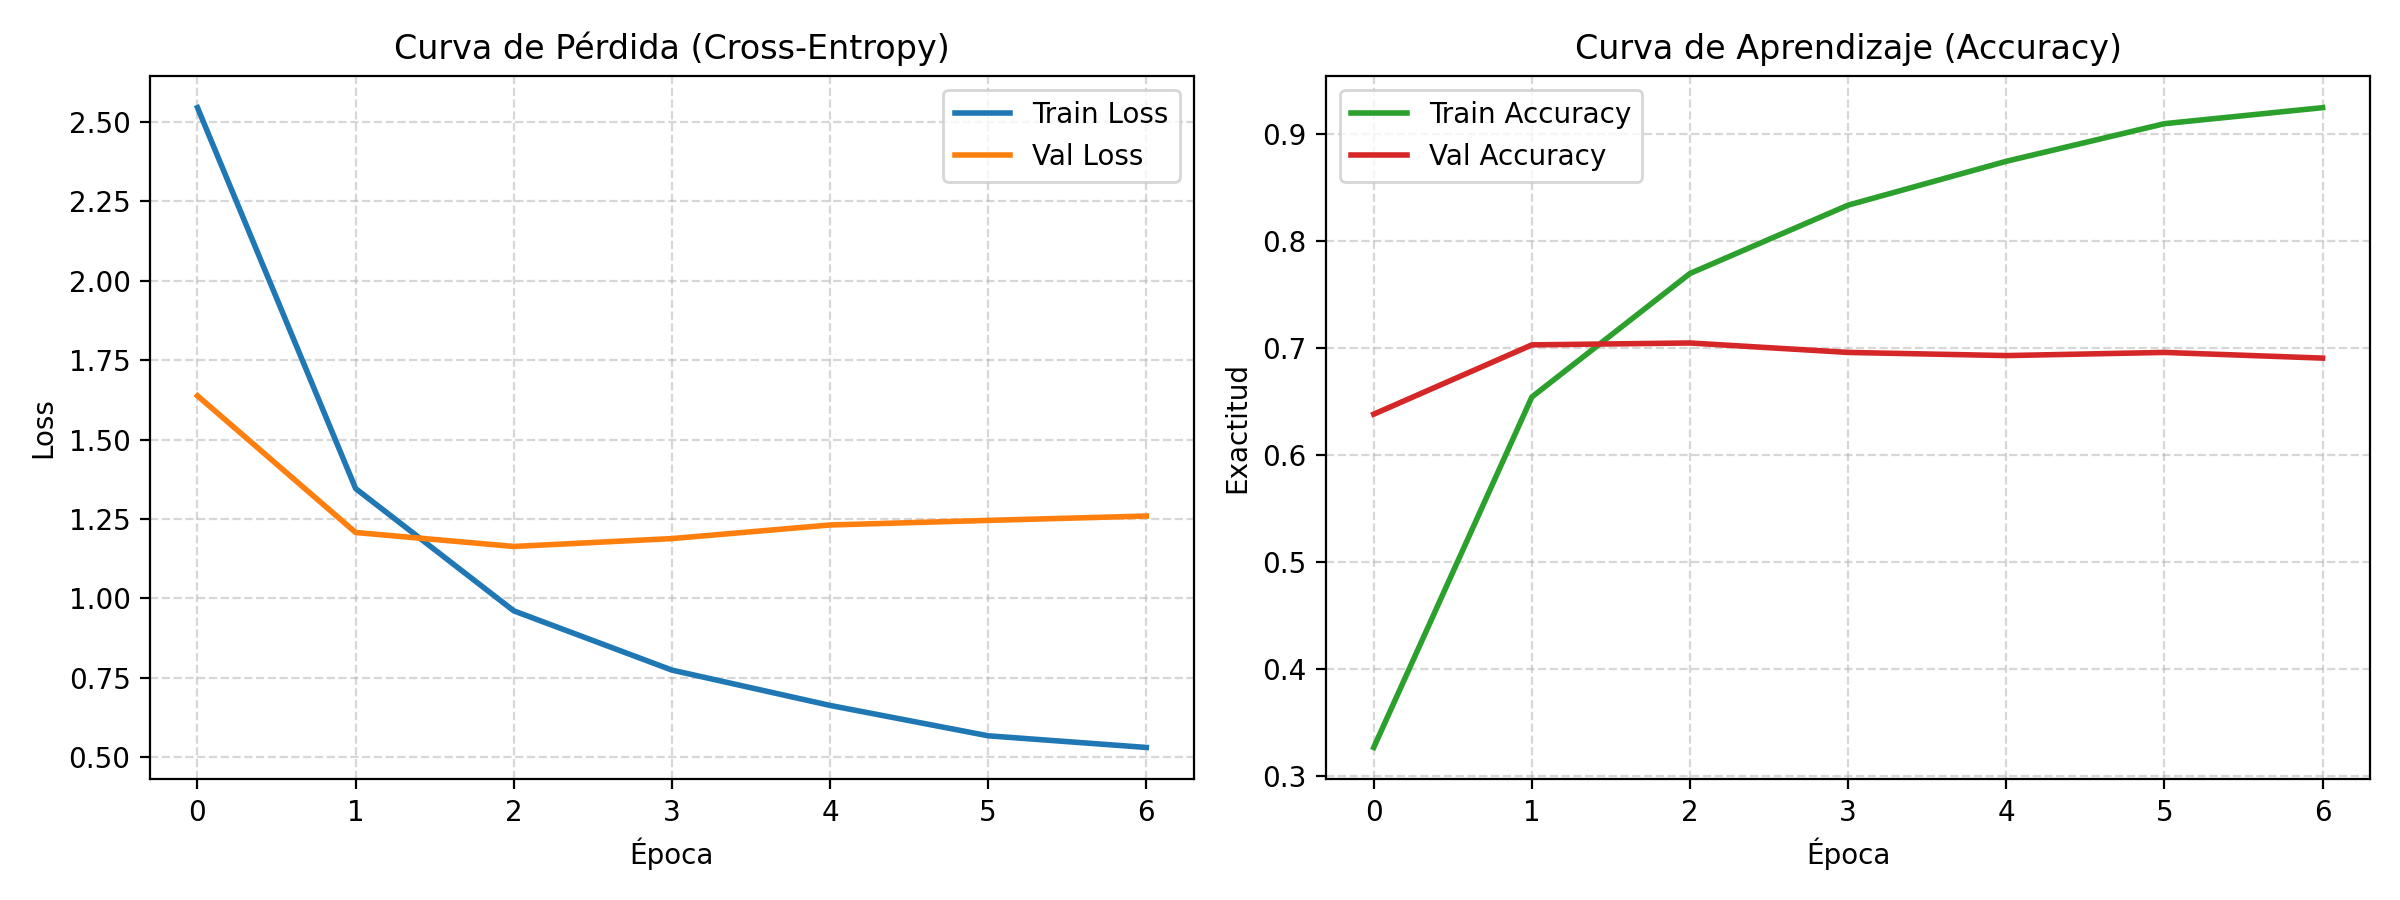
\includegraphics[width=0.98\textwidth]{learning_curves_baseline_mlp.png}
    \caption{Curvas de aprendizaje del modelo MLP Baseline: Curva de Pérdida (\textit{Loss}) a la izquierda y Curva de Exactitud (\textit{Accuracy}) a la derecha, contrastando Entrenamiento versus Validación.}
    \label{fig:learning_curves}
\end{figure}

\begin{figure}[H]
    \centering
    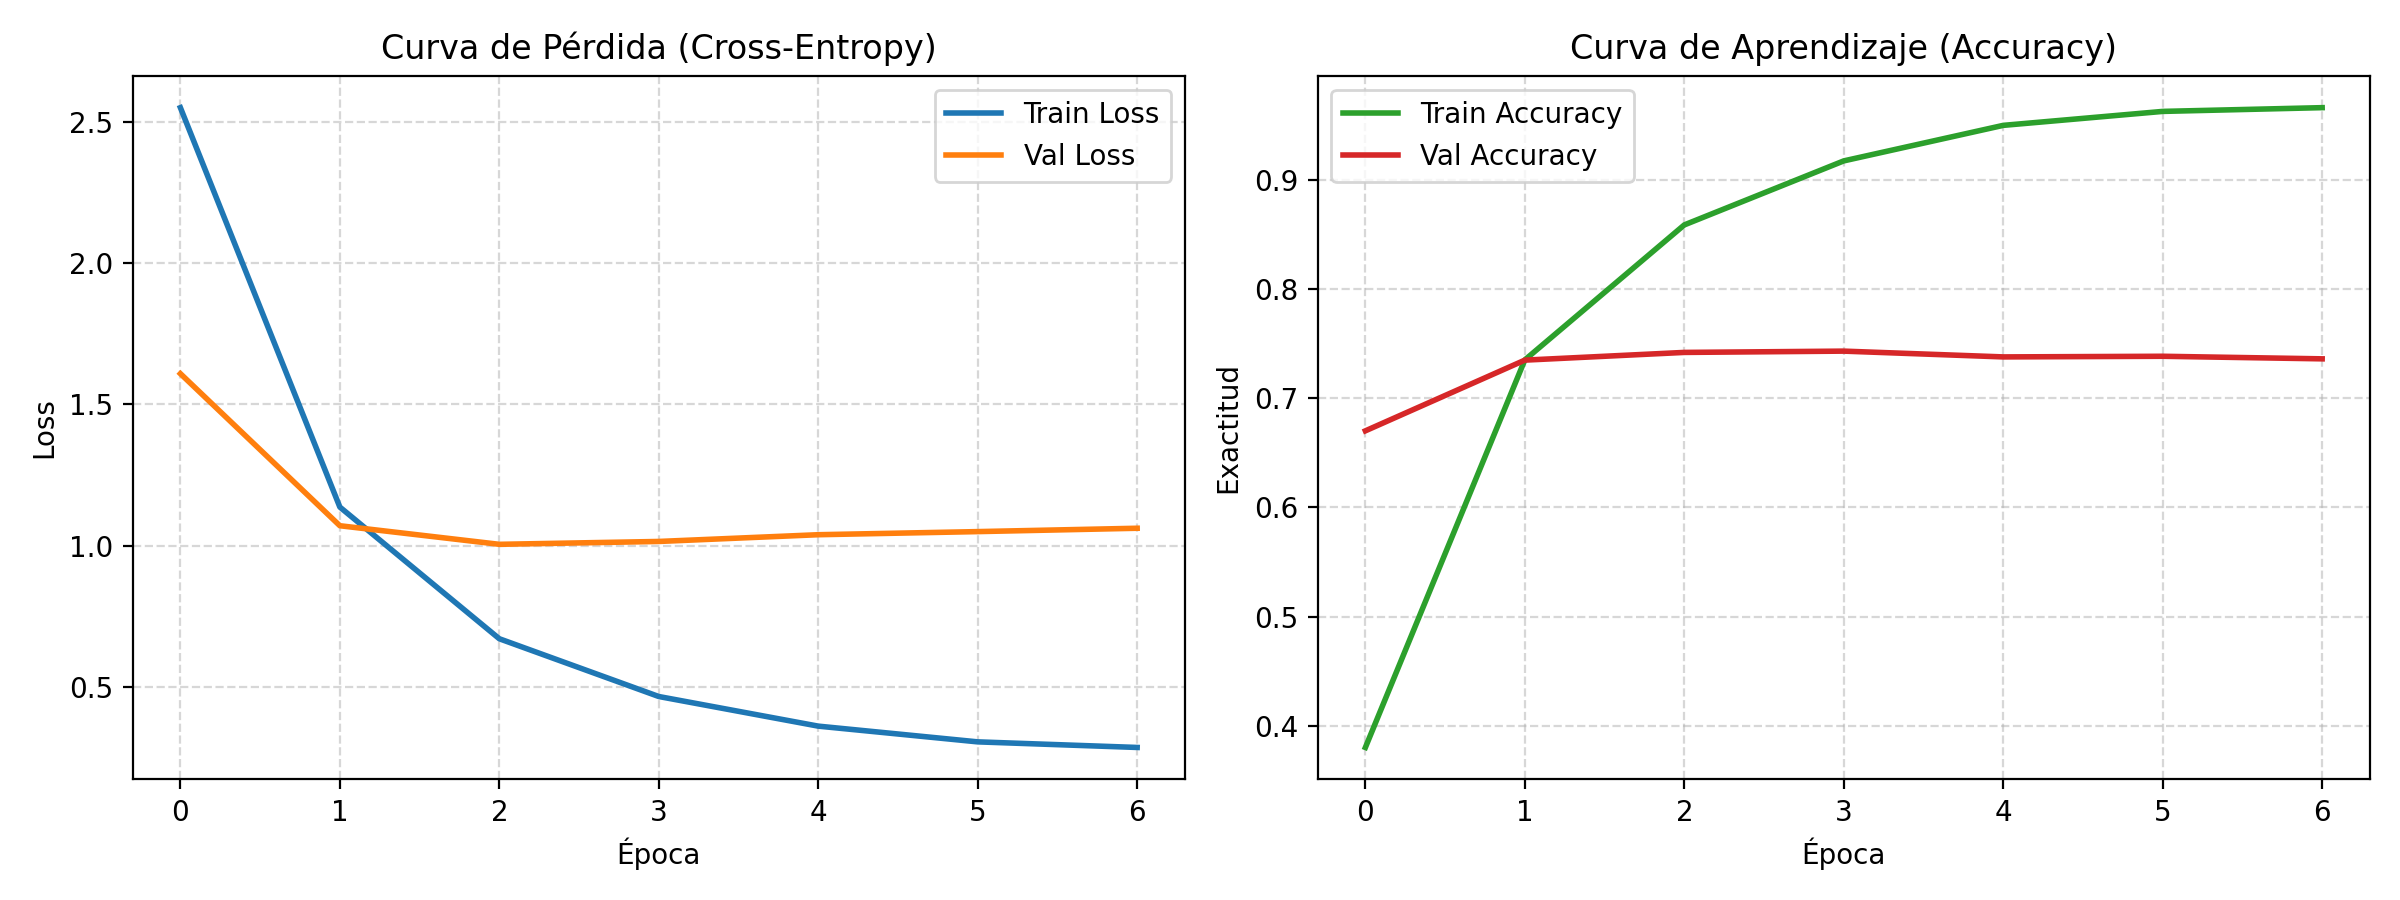
\includegraphics[width=0.98\textwidth]{learning_curves_tuned_mlp.png}
    \caption{Curvas de aprendizaje del modelo MLP Tuned, con la misma disposición que la Figura~\ref{fig:learning_curves}.}
    \label{fig:learning_curves_tuned}
\end{figure}

Del análisis detallado de las Figuras~\ref{fig:learning_curves} y~\ref{fig:learning_curves_tuned} se desprenden los siguientes hallazgos:
\begin{enumerate}
    \item \textbf{Comportamiento de la Pérdida:} En las primeras épocas se observa una caída pronunciada del costo tanto en entrenamiento como en validación, demostrando que la red extrae rápidamente las palabras clave más deterministas de cada categoría.
    \item \textbf{Control de Divergencia:} En la época $3$ (índice $2$ en el eje de la figura, que numera desde $0$) la pérdida de validación (\textit{val\_loss}) alcanza su mínimo ($\approx 1.16$) y a partir de ahí asciende levemente hasta $\approx 1.26$ en la época $7$, mientras la pérdida de entrenamiento sigue descendiendo y la exactitud de entrenamiento llega al $92\%$ frente a un $69\%$ en validación: una señal de sobreajuste incipiente. El ascenso es gradual y no abrupto; durante este tramo actúan el Dropout de $0.40$ y \texttt{ReduceLROnPlateau}, que reduce la tasa de aprendizaje a la mitad en las épocas $5$ y $7$.
    \item \textbf{Criterio de Parada y Mejor Checkpoint:} El callback \texttt{EarlyStopping} detecta el ascenso, detiene el entrenamiento en la época $7$ y restaura los pesos correspondientes al punto donde la pérdida de validación alcanzó su valor mínimo (época $3$), garantizando que el modelo exportado a disco posea la máxima capacidad de generalización.
    \item \textbf{Comparación con el Tuned:} El modelo Tuned sigue el mismo patrón: su pérdida de validación también alcanza el mínimo en la época $3$ y la parada temprana detiene el entrenamiento en la época $7$. Su mínimo es más bajo ($\approx 1.00$ frente a $\approx 1.16$), lo que coincide con su mayor exactitud en prueba. En la época $7$ sus dos exactitudes son más altas que las del Baseline ($\approx 97\%$ en entrenamiento y $\approx 74\%$ en validación, frente a $92\%$ y $69\%$), pero la brecha entre ellas es prácticamente la misma, de unos $23$ puntos.
\end{enumerate}

\subsection{Costo Computacional y Eficiencia}

La Tabla~\ref{tab:computational_cost} resume los costos temporales y espaciales del proceso experimental.

\begin{table}[H]
    \centering
    \caption{Costo computacional de ambas configuraciones, medido en el mismo equipo (CPU, sin aceleración por GPU).}
    \label{tab:computational_cost}
    \begin{tabular}{@{}lcc@{}}
        \toprule
        \textbf{Métrica de Cómputo} & \textbf{MLP Baseline} & \textbf{MLP Tuned} \\
        \midrule
        Tamaño de Vocabulario ($V$)          & 5\,000 términos & 10\,000 términos \\
        Parámetros Entrenables               & 1\,315\,732      & 5\,256\,980 \\
        Épocas Ejecutadas (mejor época)      & 7 (3)          & 7 (3) \\
        Tiempo por Época de Entrenamiento    & 5.0 seg.       & 19.1 seg. \\
        Tiempo Total de Entrenamiento        & 34.8 seg.      & 133.4 seg. \\
        \bottomrule
    \end{tabular}
\end{table}

A diferencia de los modelos profundos basados en mecanismos de atención o recurrencia (que requieren aceleración masiva en GPU durante horas), el Perceptrón Multicapa alimentado por TF-IDF se entrena en CPU en unos $35$ segundos (Baseline) y en poco más de $2$ minutos (Tuned). La mejora de $3.57$ puntos de exactitud del Tuned tiene un costo de $4$ veces más parámetros y $3.8$ veces más tiempo de entrenamiento.

\subsection{Análisis de Comportamiento en la Demostración Ejecutable}

En cumplimiento de los requerimientos de la rúbrica para la sustentación oral, se integró una rutina interactiva de inferencia que evalúa el comportamiento probabilístico ante dos tipos de oraciones. Las cifras siguientes corresponden al modelo Baseline, que es el que la demo carga por defecto:

\begin{enumerate}
    \item \textbf{Casos Claros (Alta Confianza):} Frases con términos unívocos de dominio (e.g., \textit{``NASA rover detects evidence of liquid water and atmosphere on Mars''}) obtienen una masa de probabilidad superior al $95\%$ concentrada en la categoría \texttt{sci.space}.
    \item \textbf{Casos Mixtos o Fronterizos (Confianza Promedio):} Frases que solapan conceptos de múltiples áreas exhiben una distribución repartida y competitiva entre las categorías relevantes:
    \begin{itemize}
        \item \textit{``A debate on whether doctors should perform experimental medical treatments when religious beliefs oppose it:''} La red distribuye la probabilidad entre \texttt{sci.med} ($66.9\%$), \texttt{alt.atheism} ($11.6\%$) y \texttt{talk.religion.misc} ($7.5\%$).
        \item \textit{``I installed a new operating system on my PC to play baseball and hockey video games:''} La masa probabilística se disputa entre \texttt{rec.sport.hockey} ($77.3\%$), \texttt{rec.sport.baseball} ($18.4\%$) y, en menor medida, \texttt{misc.forsale} ($3.7\%$).
    \end{itemize}
\end{enumerate}
Con el modelo Tuned, las mismas frases mixtas obtienen distribuciones más concentradas en la clase principal (\texttt{sci.med} con $79.2\%$ y \texttt{rec.sport.hockey} con $81.9\%$). Este comportamiento probabilístico refleja que la red combina la evidencia léxica de varios temas en lugar de operar como una simple tabla asociativa rígida.

% ============================================================
\section{Discusión Crítica}
% ============================================================

\textbf{Capacidad y Límites de la Representación Vectorial Estática:} \\
El Perceptrón Multicapa procesa el texto a través de una bolsa de palabras ponderada (\textit{Bag-of-Words} con TF-IDF). Aunque este enfoque es computacionalmente eficiente y captura eficazmente la presencia de palabras discriminantes, adolece de una limitación teórica: la insensibilidad al orden sintáctico y a la semántica contextual profunda. Por ejemplo, las oraciones \textit{``The doctor treated the patient without medicine''} y \textit{``The patient treated the doctor without medicine''} proyectan representaciones vectoriales prácticamente indistinguibles en TF-IDF, a pesar de que su significado relacional es completamente opuesto.

\textbf{El Compromiso entre Dimensionalidad y Generalización:} \\
El tamaño del vocabulario $V$ determina directamente la dimensión de entrada y, por ende, la cantidad de pesos de la primera capa oculta ($V \times 256$ en el Baseline y $V \times 512$ en el Tuned). Ampliar el vocabulario más allá de cierto umbral puede introducir palabras con frecuencias extremadamente bajas en el corpus, lo que incrementa el riesgo de que las conexiones densas se ajusten a idiosincrasias particulares de muestras individuales en lugar de patrones universales. En los experimentos, pasar de $5\,000$ a $10\,000$ términos, junto con una primera capa de $512$ neuronas y una regularización más moderada, elevó la exactitud en $3.57$ puntos; la brecha entre entrenamiento y validación se mantuvo en unos $23$ puntos y ambos modelos sobreajustan desde la época $3$, de modo que el beneficio también depende de la parada temprana. Como los cinco hiperparámetros se modificaron a la vez, estos experimentos no permiten atribuir la mejora a uno de ellos en particular. Tampoco se evaluaron vocabularios mayores a $10\,000$ términos, por lo que estos resultados no permiten afirmar en qué punto se satura la mejora.

\textbf{Validez de la Evaluación sin Metadatos:} \\
Haber suprimido rigurosamente los encabezados y firmas representa una fortaleza metodológica del proyecto. Si bien reportar precisiones superiores al $80\%$ incorporando cabeceras de correo puede parecer más atractivo superficialmente, dicho resultado es espurio y carece de validez técnica. La exactitud de $68.03\%$ alcanzada en este reporte constituye una medición genuina de la capacidad del modelo para discernir temas basándose en el cuerpo narrativo del texto.

% ============================================================
\section{Conclusiones}
% ============================================================

A partir del desarrollo, experimentación y análisis cuantitativo de la Entrega 1, se concluye que:

\begin{enumerate}
    \item El Perceptrón Multicapa (MLP) acoplado a representaciones normalizadas de \textbf{TF-IDF} es una arquitectura funcional y eficiente para la clasificación multiclase de texto en 20 Newsgroups: la configuración Tuned alcanza una exactitud de $68.03\%$ y un $F_1$-score macro de $66.90\%$ en el conjunto de prueba independiente, unas $13.6$ veces el acierto esperado al azar ($5\%$).
    \item La remoción de metadatos de cabecera y firma es un paso imprescindible para evitar el fenómeno de fuga de información (\textit{data leakage}), permitiendo evaluar la generalización real de la red sobre el contenido semántico de las noticias.
    \item Con activaciones \textbf{ReLU} en las capas densas intermedias, ambas configuraciones convergen rápidamente (el mínimo de la pérdida de validación se alcanza en la época $3$), mientras que la función \textbf{Softmax} en la salida modeló de forma rigurosa la distribución de probabilidades de las $20$ clases mutuamente excluyentes.
    \item La parada temprana (\textit{EarlyStopping}) determina qué pesos conserva el modelo final: en ambas configuraciones la pérdida de validación asciende desde la época $3$ y la parada temprana recupera los pesos de ese punto, evitando que el modelo final arrastre el sobreajuste propio de entradas dispersas de alta dimensionalidad. El Dropout y la penalización $L_2$, por sí solos, no impiden ese ascenso.
    \item Ampliar el vocabulario a $10\,000$ términos y la primera capa a $512$ neuronas, con una regularización más moderada, mejoró la exactitud en $3.57$ puntos y el $F_1$ macro en $3.94$ puntos. La mejora es consistente entre semillas ($67.9 \pm 0.3\%$ frente a $64.9 \pm 0.7\%$) y tiene un costo de $4$ veces más parámetros y $3.8$ veces más tiempo de entrenamiento. Dado que se modificaron cinco hiperparámetros a la vez, queda pendiente aislar cuál de ellos aporta la mayor parte de la mejora.
    \item La demostración interactiva desarrollada evidencia que el modelo asigna de forma consistente distribuciones de probabilidad repartidas cuando se enfrenta a textos de dominios mixtos o fronterizos, corroborando un aprendizaje coherente de las relaciones léxicas.
\end{enumerate}

% ============================================================
%  BIBLIOGRAFÍA
% ============================================================
\newpage
\begin{thebibliography}{9}

\bibitem{lang1995newsweeder}
Lang, K. (1995).
Newsweeder: Learning to filter netnews.
En \textit{Proceedings of the Twelfth International Conference on Machine Learning} (pp. 331--339).

\bibitem{chollet2021deep}
Chollet, F. (2021).
\textit{Deep Learning with Python} (2da ed.).
Manning Publications.

\bibitem{pedregosa2011scikit}
Pedregosa, F., Varoquaux, G., Gramfort, A., Michel, V., Thirion, B., Grisel, O., Blondel, M., Prettenhofer, P., Weiss, R., Dubourg, V. y Vanderplas, J. (2011).
Scikit-learn: Machine Learning in Python.
\textit{Journal of Machine Learning Research}, 12, 2825--2830.


\end{thebibliography}

\end{document}
